\section{Web-Components}
\label{sec:3_Web_Components}

\todo[inline]{HTML Templates W3C Draft (18.März.2014) https://dvcs.w3.org/hg/webcomponents/raw-file/tip/spec/templates/index.html}
%http://www.w3.org/TR/html5/scripting-1.html#the-template-element

Um Web-Components besser verstehen zu können, wird in diesem Kapitel zu Beginn eine kurze Übersicht über die Geschichte von Web-Bibliotheken gezeigt.

\begin{description}
\item[2005] Veröffentlichung von Dojo Toolkit\footnote{Mehr Information zu Dojo Toolkit auf \href{http://dojotoolkit.org/}{http://dojotoolkit.org/}} mit der innovativen Idee von Widgets. Mit ein paar Zeilen Code konnten Entwickler komplexe Elemente, wie beispielsweise einen Graph oder eine Dialog-Box in ihrer Website hinzufügen.
\item[2006] jQuery\footnote{Mehr Information zu jQuery auf \href{http://jquery.com/}{http://jquery.com/}} stellt Entwicklern die Funktion zur Verfügung Plugins zu entwickeln, die später wiederverwendet werden können.
\item[2008] Veröffentlichung von jQuery UI\footnote{Mehr Information zu jQuery UI auf \href{http://jqueryui.com/}{http://jqueryui.com/}}, was vordefinierte Widgets und Effekte mit sich bringt.
\item[2009] Erstveröffentlichung von AngularJS\footnote{Mehr Information zu AngularJS auf \href{http://angularjs.org/}{http://angularjs.org/}}, ein Framework mit Direktiven.
\item[2011] Erstveröffentlichung von React\footnote{Mehr Information zu Facebook React auf \href{http://facebook.github.io/react/}{http://facebook.github.io/react/}}. Diese Bibliothek gibt den Entwicklern die Fähigkeit, das User Interface ihrer Website zu bauen, ohne dabei auf andere Frameworks, die auf der Seite benutzt werden, achten zu müssen
\item[2013] Veröffentlichung des Entwurfs von Web-Components, jedoch mit schlechter Browser Unterstützung
\end{description}

Mit der Veröffentlichung von Dojo Toolkit sagen Entwickler die Vorteile von wiederverwendbaren Modulen. Wenn man zurzeit Plugins auf einer Website erwähnt, denken die meisten Entwickler von jQuery Plugins, da sie beinahe überall Verwendung finden und ein großes Spektrum von Funktionen bieten. Mit den Veröffentlichungen von AngularJS und React wurde gezeigt, in welche Richtung sich Web-Anwendungen bewegen. Sie zeigen, dass es nicht nur um visuelle Elemente geht, sondern auch um Elemente, die eine komplexe Logik besitzen.




Ähnlich zu HTML5 ist Web-Components ein Sammelbegriff für mehrere Features:
\begin{description}
\item[Shadow DOM (ausführliche Erklärung siehe Kapitel \ref{sec:3_WC_Shadow_DOM} auf Seite \pageref{sec:3_WC_Shadow_DOM})] erlaubt es das DOM und CSS zu kapseln
\item[HTML Templates (ausführliche Erklärung siehe Kapitel \ref{sec:3_WC_Templates} auf Seite \pageref{sec:3_WC_Templates})] sind ein Weg, um den DOM zu klonen und somit den Klon wiederzuverwenden
\item[Custom Elements (ausführliche Erklärung siehe Kapitel \ref{sec:3_WC_Elements} auf Seite \pageref{sec:3_WC_Elements})] können einerseits neue Elemente definieren, oder bereits bestehende Elemente erweitern. Dies bedeutet, dass ein Entwickler beispielsweise den HTMl \lstinline|<input>|-Tag dahingehend erweitern kann, dass dieser nur das Format von Kreditkartennummern unterstützt. Ein Beispiel für die Definition eines neuen Elements wäre ein Element, dass sämtliche Felder, die für die Bezahlung mit einer Kreditkarte notwendig sind, bereitstellt.
\item[HTML Imports (ausführliche Erklärung siehe Kapitel \ref{sec:3_WC_Imports} auf Seite \pageref{sec:3_WC_Imports})] sind dazu da, um externe HTML-Dateien in die bestehende Website zu integrieren, ohne dabei den Code kopieren zu müssen. Sie können beispielsweise dazu verwendet werden, um Web-Components in eine Website zu integrieren.
\item[Decorators (ausführliche Erklärung siehe Kapitel \ref{sec:3_WC_Decorators} auf Seite \pageref{sec:3_WC_Decorators})] sind Elemente, die nach dem \glqq Decorator-pattern\grqq\ benannt sind. Durch dieses Pattern ist es möglich Elemente um zusätzliche Funktionalitäten zur Laufzeit erweitern zu können.
\end{description}

Obwohl \glqq Web-Components\grqq\ für viele Entwickler noch kein Begriff ist, wird es bereits vom Browser automatisch verwendet. Beispiele dafür sind der Datepicker oder das \lstinline|<video>|-Elemen. Abbildung \ref{fig:3_Datepicker_Visuals} auf Seite \pageref{fig:3_Datepicker_Visuals} zeigt die Datepicker-Komponente und Abbildung \ref{fig:3_Datepicker_Source} auf Seite \pageref{fig:3_Datepicker_Source} zeigt den dazugehörigen Source-Code. Dieser Code zeigt, dass sämtliche Kontrollbuttons des Datepickers vor dem Entwickler \glqq versteckt\grqq , also im Shadow DOM liegen.


\begin{figure}[h]
\centering
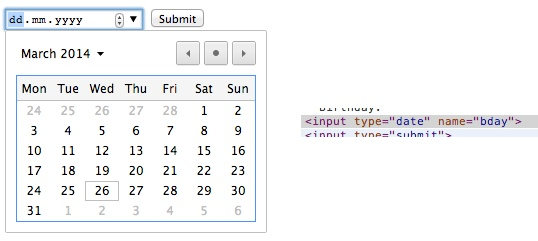
\includegraphics[height=5.0cm]{images/datepicker.jpg}
\caption[
Beispiel von Web-Components im Browser an Hand von dem Datepicker, Urldate: 04.2014 \newline
\small\texttt{https://s3.amazonaws.com/infinum.web.production/repository\_items/files/000/000/238/original/datepicker.jpg}
]{Beispiel von Web-Components im Browser an Hand von dem Datepicker}
\label{fig:3_Datepicker_Visuals}
\end{figure}

\begin{figure}[h]
\centering
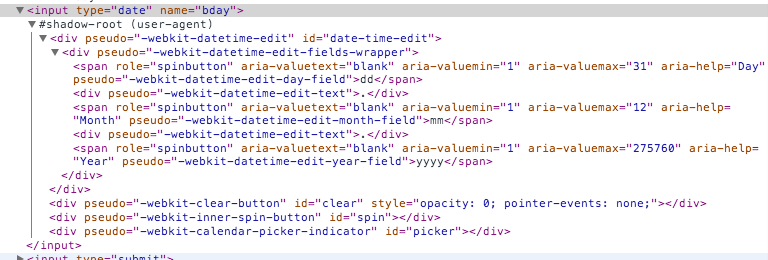
\includegraphics[height=5.0cm]{images/datepicker_shadow_dom.jpg}
\caption[
Beispiel von Web-Components im Browser an Hand von dem Datepicker, Urldate: 04.2014 \newline
\small\texttt{https://s3.amazonaws.com/infinum.web.production/repository\_items/files/000/000/236/original/datepicker\_shadow\_dom.jpg}
]{Beispiel von Web-Components im Browser an Hand von dem Datepicker}
\label{fig:3_Datepicker_Source}
\end{figure}

\textbf{Warum Web-Components?}\\
Javascript Widgets und Plugins sind fragmentiert, weil sie auf diversen unterschiedlichen Bibliotheken und Frameworks basieren, die möglicherweise nicht miteinander funktionieren. Web-Components versuchen einen gewissen Standard in Widgets und Plugins zu bringen. Das Problem der nicht miteinander funktionierenden Plugins versucht Web-Components mit Kapselung zu lösen. Durch die Lösung dieses Problems ist die Wiederverwendbarkeit von Komponenten garantiert, da es sämtliche Interferenzen zwischen Plugins löst. Web-Components können des Weiteren viel mehr als nur UI-Komponenten sein. Eine Bibliothek könnte bereits eine Komponente darstellen, die eine gewisse Funktionalität bereitstellt.

\textbf{Unterstützung von Web-Components}\\
Zur Zeit ist die Hauptproblem von Web-Components die mangelhafte Browserunterstützung. Kein einziger Browser unterstützt diesen Standard zu 100\%. Es gibt bereits mehrere Möglichkeiten beziehungsweise Polyfills\footnote{Ein Polyfill ist ein Browser-Fallback, um Funktionen, die in modernen Browsern verfügbar sind, auch in alten Browsern verfügbar zu machen.}, um dennoch Web-Components nutzen zu können. Beispiele hierfür sind:
\begin{itemize}
\item Polyfill-Webcomponents\footnote{Mehr Information zu Polyfill-Webcomponents unter \href{http://github.com/timoxley/polyfill-webcomponents}{http://github.com/timoxley/polyfill-webcomponents}}
\item Polymer-Project\footnote{Mehr Information zu Polymer unter \href{http://www.polymer-project.org/}{http://www.polymer-project.org/}}
\item X-tags\footnote{Mehr Information zu X-tags unter \href{http://x-tags.org/}{http://x-tags.org/}}
\end{itemize}
Obwohl es mehrere Polyfills bezüglich Web-Componnts gibt, ist es egal, auf welcher Basis man seine Web-Components programmiert, denn durch die Standardisierung ist die Interkompatibilität der einzelnen Komponenten gegeben. Diese Arbeit beschränkt sich hauptsächlich auf die Entwicklung von Web-Components mit Hilfe des Standards beziehungsweise der Polyfill-Bibliothek Polymer.\\
Durch die Benutzung von dem Polyfill Polymer funktionieren Web-Component in allen \glqq evergreen\grqq -Browsern\footnote{Ein \glqq Evergreen\grqq -Browser ist ein Web-Browser, der sich automatisch beim Start updatet.} und Internet-Explorer 10 und neuer. Des Weiteren funktionieren sie dadurch auf mobilen Endgeräten, wo iOS6+, Chrome Mobile, Firefox Mobile, oder Android 4.4 oder höher vorhanden ist. Auch mit Hilfe von Polyfill bieten sowohl der Internet-Explorer 9 und niedriger, als auch Android-Browser 4.3 oder niedriger keine Unterstützung für Web-Components. Dies bedeutet, dass Web-Components zur Zeit noch für die Verwendung im Web bereit sind, außer man hat als Zielgruppe ausschließlich eine Plattform, die unterstützt wird.

\textbf{Web-Components Alternativen}
Die folgenden Alternativen von Web-Components benutzen ähnliche Pattern um die gewünschte DOM-Abstrahierung zu erreichen.
\begin{description}
\item[React] benutzt seinen eigenen \glqq Virtual DOM\grqq und versucht in keinster Hinsicht Web-Components zu simulieren. Folglich ist die Browser-Unterstützung von React besser, als jene der Web-Components. Ab Internet-Explorer 8 werden sämtliche Browser vollständig unterstützt. Zur Zeit wird diese Technologie in Facebooks und Instagrams Kommentarsystemen eingesetzt.
\item[AngularJS] besitzt diverse Interferenzen zu Web-Components, jedoch versucht auch diese Technologie nicht Web-Components zu simulieren, um bessere Browser-Unterstützung zu bieten (Internet Explorer 8+). Die genaue Unterscheidung bezüglich AngularJS-Direktiven und Web-Components werden in Kapitel \ref{sec:3_Polymer} auf Seite \pageref{sec:3_Polymer} erklärt.
\end{description}



%\subsection{Relevanz von Web-Components hinsichtlich der Forschungsfrage}
%\label{sec:3_Relevanz}

\subsection{W3C Web-Components Standard}
\label{sec:3_W3C}

\subsubsection{Templates}
\label{sec:3_WC_Templates}

Das folgende Kapitel basiert ausschließlich auf der Spezifikation von Templates des W3C \citereset \autocite[siehe][]{Weinstein.2013} und auf dem Artikel \glqq HTML's new Template Tag\grqq\ \citereset \autocite[siehe][]{BidelmanTemplate.2013}.

Laut W3C sind Templates
\begin{quote}
\glqq
  a method for declaring inert DOM subtress in HTML and manipulating them to instantiate document fragments with identical contents.
\grqq
\end{quote}
Somit sind Templates eine Methode um inaktive DOM-Unterstruktur in HTML zu deklarieren und zu manipulieren, um so sämtliche identische Dokumentfragmente mit identischem Inhalt zu instanziieren.

In Web-Applikationen wird oft die gleiche Unterstruktur von Elementen wiederverwendet, mit dem passenden Inhalt gefüllt und zum Dokument hinzugefügt. Ein Beispiel in disem Kontext wäre eine Liste von Artikel, die mit mehreren \lstinline|<li>| -Tags in das Dokument eingefügt werden. Des Weiteren kann jeder \lstinline|<li>|-Tag weitere Elemente, wie beispielsweise einen Link, ein Bild, einen Paragraphen, etc., enthalten. Derzeit bot HTML keine native Möglichkeit an, eine solche Aufgabenstellung zu lösen.

Folgend wird eine Liste von Autos mit Hilfe eines Templates erstellt:
\begin{lstlisting}[language=HTML, caption={Web-Components Template-Standard}, label={lst:3_Templates}, escapeinside={@}{@}]
<template id="carTemplate">
  <li>
    <span class="carBrand"></span>
    <span class="carName"></span>
  </li>
</template>
\end{lstlisting}

Ein Template, wie das aus Code-Beispiel \ref{lst:3_Templates} auf Seite \pageref{lst:3_Templates}, kann sowohl im \lstinline|<head>|- als auch im \lstinline|<body>| definiert werden. Das Template, inklusive Subtree, ist inaktiv. Wenn sich ein \lstinline|<img>|-Tag mit einer validen Quelle in diesem Template befinden würde, würde der Browser dieses Bild nicht laden. Darüber hinaus ist es nicht möglich ein Element des Templates via JavaScript zu selektieren, wie in Code-Beispiel \ref{lst:3_Selector_Example} auf Seite \pageref{lst:3_Selector_Example} gezeigt wird.

\begin{lstlisting}[language=JavaScript, caption={Beispiel-Selektor eines Elements in einem Template, das nicht aktiven DOM ist}, label={lst:3_Selector_Example}]
  document.querySelectorAll('.carBrand').length; // length ist 0
\end{lstlisting}

\begin{figure}[h]
\centering
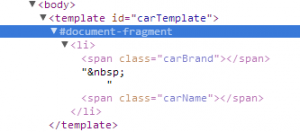
\includegraphics[height=3.0cm]{images/document_fragment.png}
\caption[
Visualisierung des DOM eines inaktiven Templates, Urldate: 04.2014
\newline
\small\texttt{\url{http://www.prevent-default.com/wp-content/uploads/2013/04/document-fragment-300x132.png}}
]{Visualisierung des DOM eines inaktiven Templates}
\label{fig:3_inactive_Template_DOM}
\end{figure}

In Abbildung \ref{fig:3_inactive_Template_DOM} auf Seite \pageref{fig:3_inactive_Template_DOM} wird gezeigt, dass das Template ein Dokument-Fragment ist. Dies bedeutet, dass es ein eigenständiges Dokument ist und unabhängig vom ursprünglichen Dokument existiert. Folglich bedeutet dies, dass sämtliche \lstinline|<script>, <form>, <img>, |-Tags etc. nicht verwendet werden können.

\begin{lstlisting}[language=JavaScript, caption={Verwendung des Templates \ref{lst:3_Templates} auf Seite \pageref{lst:3_Templates}}, label={lst:3_Templates_Verwendung}, escapeinside={@}{@}]
@\label{lst:3_Templates_Verwendung_1}@var template = document.getElementById('carTemplate');
template.content.querySelector(".carBrand").length; // length ist 1

@\label{lst:3_Templates_Verwendung_2}@var car = template.content.cloneNode(true);
car.querySelector(".carBrand").innerHTML = "Seat";
car.querySelector(".carName").innerHTML = "Ibiza";

@\label{lst:3_Templates_Verwendung_3}@document.getElementById("carList").appendChild(car);
\end{lstlisting}

Code-Beispiel \ref{lst:3_Templates_Verwendung} auf Seite \pageref{lst:3_Templates_Verwendung} basiert auf dem in Code-Beispiel \ref{lst:3_Templates} auf Seite \pageref{lst:3_Templates} definierten Template. Zu Beginn wird sich in Zeile \ref{lst:3_Templates_Verwendung_1} des Code-Beispiels \ref{lst:3_Templates_Verwendung} das bereits definierte Template in die Variable \lstinline|template| geholt. Daraufhin wird der gesamte Knoten in Zeile \ref{lst:3_Templates_Verwendung_2} mit Hilfe einer \lstinline|deep-copy| geklont und folglich mit Daten befüllt. Damit das mit Daten befüllte Listenelement auch sichtbar wird, wird es in Zeile \ref{lst:3_Templates_Verwendung_3} in das aktive DOM eingefügt.


\subsubsection{Decorators}
\label{sec:3_WC_Decorators}
Das folgende Kapitel basiert ausschließlich auf der Einführung zu Web-Components aus dem W3C \citereset \autocite{Glakov.2013}.

Decorators sind Elemente, die nach dem Decorator-Pattern benannt sind. Zur Zeit gibt es keinerlei Unterstützung von Seiten der Browser zu diesem Konzept, somit wird in dieser Arbeit das vom W3C definierte Konzept nur theoretisch erläutert. Um jedoch dieses Konzept verstehen zu können muss zuerst das genannte Pattern kurz beschrieben werden.

Grundsätzlich gehört das Decorator-Pattern zu den Struktur-Pattern der Softwareentwicklung. Das Pattern ist eine flexible Alternative zur Unterklassenbildung, um eine Klasse zur Laufzeit um zusätzliche Funktionalitäten erweitern zu können. Hinsichtlich der Verwendung des Patterns und dem Dekorator-Konzept bringt dies kleine Vorteile mit sich. Sie bestehen beispielsweise darin, dass mehrere Dekorierer hintereinandergeschaltet werden können. Weiters ist die Laufzeitbeeinflussung der Dekorierer als Vorteil zu sehen, da sie ausgetauscht werden können. Folglich kann Funktionalität eines individuellen Objekts zur Laufzeit erweitert werden, ohne dabei die Funktionalität von anderen Objekten der selben Klasse zu ändern.

Um Decorators mit Hilfe des W3C-Konzepts näher erklären zu können, wird in diesem Kapitel folgendes Beispiel verwendet. Es gibt eine Liste von Autos, wobei jedes Auto
eine Modellbezeichnung, eine Marke, ein Bild, sowie eine Kurzbeschreibung hat. Das Markup eines Autos würde wie folgt aussehen:

\begin{lstlisting}[language=HTML, caption={Web-Components Decorators - Markup eines Autos}, label={lst:3_Decorators_Basic}, escapeinside={@}{@}]
<li class="car-item">
   <img class="car-image" title="Seat Ibiza" src="images/seat-ibiza.jpg" />
   <h3 class="car-model">Seat Ibiza</h3>
   <p class="car-description">The SEAT Ibiza is a supermini car manufactured by the Spanish automaker SEAT. It is SEAT&#039;s best-selling car and perhaps the most popular model in the company&#039;s range.</p>
</li>
\end{lstlisting}

Unter der Annahme, dass man das Bild des Autos um die Funktionalität erweitern will, sodass man es sichtbar machen, unsichtbar machen beziehungsweise schließen kann, würde man das bereits vorhandene Markup aus Listing \ref{lst:3_Decorators_Basic} auf Seite \pageref{lst:3_Decorators_Basic} wie folgt erweitern:

\begin{lstlisting}[language=HTML, caption={Web-Components Decorators - Markup eines Autos mit Rahmen}, label={lst:3_Decorators_Basic2}, escapeinside={@}{@}]
<li class="car-item">
   <section class="window-frame">
      <header>
          <a class="frame-toggle" href="#">Min/Max</a>
          <a class="frame-close" href="#">Close</a>
      </header>
      <img class="car-image" title="Seat Ibiza" src="images/seat-ibiza.jpg" />
      <h3 class="car-model">Seat Ibiza</h3>
      <p class="car-description">The SEAT Ibiza is a supermini car manufactured by the Spanish automaker SEAT. It is SEAT&#039;s best-selling car and perhaps the most popular model in the company&amp;#039;s range.</p>
   </section>
</li>
\end{lstlisting}

Listing \ref{lst:3_Decorators_Basic2} auf Seite \pageref{lst:3_Decorators_Basic2} würde somit das Markup eines Autos beinhalten, wobei es zwei Buttons gibt: einen zum Umschalten zwischen sichtbar und unsichtbar und einen um das Bild komplett zu löschen.
Wenn man es mit den bisherigen standardisierten Möglichkeiten umsetzt, wird der Quellcode schnell aufgebläht.

Decorators würden in diesem Beispiel bereits helfen. Man könnte definieren, dass spezielle Elemente im DOM mit mehr Markup, Style und zusätzlicher Funktionalität versehen werden. Essentiell hierbei ist, dass es möglich ist die Basisfunktionalität nur für eine gewünschte Menge an Elementen erweitern zu können. Wenn man die erweiterte Funktionalität des Auto-Beispiels mit Hilfe von Decorators umsetzen würde, würde es wie folgt aussehen:

\begin{lstlisting}[language=HTML, caption={Web-Components Decorators - Markup der zusätzlichen Funktionalität (Rahmen)}, label={lst:3_Decorators_Basic3}, escapeinside={@}{@}]
<decorator id="frame-decorator">
   <template>
      <section id="window-frame">
         <header>
            <a id="toggle" href="#">Min/Max</a>
            <a id="close" href="#">Close</a>
         </header>
         @\label{lst:3_Decorators_Basic3_content}@<content></content>
      </section>
   </template>
</decorator>
\end{lstlisting}

Dieses Beispiel bedarf näherer Erklärung. Decorators werden grundsätzlich mit \lstinline|<template>|-Elementen eingesetzt (mehr zu Templates in Kapitel \ref{sec:3_WC_Templates} auf Seite \pageref{sec:3_WC_Templates}). Des Weiteren wird in Zeile \ref{lst:3_Decorators_Basic3_content} der Listing \ref{lst:3_Decorators_Basic3} ein \lstinline|<content>|-Element verwendet. Dies ist zwingend notwendig, da in dieser Stelle der Inhalt des zu dekorierenden Elements eingefügt wird. Auch ist zu erwähnen, dass in diesem Beispiel nur \lstinline|id|s verwendet werden, was nicht zu empfehlen ist. Jedoch sollte es zur Visualisierung dienen, dass \lstinline|id|s innerhalb eines \lstinline|<decorator>|-Elements gekapselt sind. Sie werden nie im DOM erscheinen beziehungsweise verfügbar sein. \lstinline|document.getElementById("window-frame")| wird keine Elemente zurückgeben, weder vor noch nach der Anwendung des \lstinline|<decorator>|-Elements.

Weiterhin ist es möglich, sämtliche Elemente eines Decorators zu gestalten. In Listing \ref{lst:3_Decorators_Basic4} auf Seite \pageref{lst:3_Decorators_Basic4} werden die beiden Buttons mit \lstinline|float: right;| gestaltet. Um die \lstinline|floats| der Elemente wieder zu löschen, wird das \lstinline|<header>|-Element mit der CSS-Klasse \lstinline|clearfix| erweitert.

\begin{lstlisting}[language=HTML, caption={Web-Components Decorators - Markup der zusätzlichen Funktionalität (Rahmen) inklusive Style}, label={lst:3_Decorators_Basic4}, escapeinside={@}{@}, escapechar=!]
<decorator id="frame-decorator">
   <template>
      <section id="window-frame">
        !\colorbox{light-gray}{<style scoped>}!
            !\colorbox{light-gray}{\#toggle {float: right;}}!
            !\colorbox{light-gray}{\#close {float: right;}}!
         !\colorbox{light-gray}{</style>}!
         !\colorbox{light-gray}{<header class="clearfix">}!
            <a id="toggle" href="#">Min/Max</a>
            <a id="close" href="#">Close</a>
         </header>
         <content></content>
      </section>
   </template>
</decorator>
\end{lstlisting}

Es ist zu beachten, dass sämtliche Gestaltungen außerhalb des \lstinline|<style scoped>|-Elements unter Verwendung der richtigen Klassennamen immer noch angewendet werden.

Um nun das bereits vorhandene Markup mit Funktionalität versehen zu können, muss zuerst noch etwas erläutert werden\todo{umschreiben}. Bei Decorators gibt es keine \glqq normalen\grqq\ Events, wie man es gewöhnt ist. Das Hinzufügen beziehungsweise Entfernen eines Decorators würde das Event, wenn es auf ein Element gebunden war, löschen. Anstatt normalen Events hat man mit Hilfe von Decorators die Möglichkeit einen Event-Controller zu erstellen, um mittels diesen Events verwalten zu können.

\begin{lstlisting}[language=HTML, caption={Web-Components Decorators - Markup der zusätzlichen Funktionalität (Rahmen) inklusive Style und Funktionalität}, label={lst:3_Decorators_Basic5}, escapeinside={@}{@}, escapechar=!]
<decorator id="frame-decorator">
   <script>
      this.listen({
         selector:"#toggle", type:"click",
         handler: function (event) {
            // do the toggle button logic here
         }
      });
      this.listen({
         selector:"#close", type:"click",
         handler: function (event) {
            // do the close button logic here
         }
      });
   </script>
   <template>
      <section id="window-frame">
         <style scoped>
            #toggle {float: right;}
            #close {float: right;}
         </style>
         <header class="clearfix">
            <a id="toggle" href="#">Min/Max</a>
            <a id="close" href="#">Close</a>
         </header>
         <content></content>
      </section>
   </template>
</decorator>
\end{lstlisting}


Der in Listing \ref{lst:3_Decorators_Basic5} auf Seite \ref{lst:3_Decorators_Basic5} gezeigte Decorator kann somit verwendet werden, um die gewünschte Funktionalität (das Bild des Autos soll sichtbar, unsichtbar beziehungsweise gelöscht werden können) bereitstellen zu können, ohne dabei für jedes \lstinline|<li>|-Element extra Markup hinzufügen zu müssen. Schlussendlich würde das Beispiel für ein Auto wie folgt aussehen:

\begin{lstlisting}[language=HTML, caption={Web-Components Decorators - Markup eines Autos mit Decorator}, label={lst:3_Decorators_Basic6}, escapeinside={@}{@}, escapechar=!]
<decorator id="frame-decorator">
   <script>
      this.listen({
         selector:"#toggle", type:"click",
         handler: function (event) {
            // do the toggle button logic here
         }
      });
      this.listen({
         selector:"#close", type:"click",
         handler: function (event) {
            // do the close button logic here
         }
      });
   </script>
   <template>
      <section id="window-frame">
         <style scoped>
            #toggle {float: right;}
            #close {float: right;}
         </style>
         <header class="clearfix">
            <a id="toggle" href="#">Min/Max</a>
            <a id="close" href="#">Close</a>
         </header>
         <content></content>
      </section>
   </template>
</decorator>

<li class="car-item">
   <img class="car-image" title="Seat Ibiza" src="images/seat-ibiza.jpg" />
   <h3 class="car-model">Seat Ibiza</h3>
   <p class="car-description">The SEAT Ibiza is a supermini car manufactured by the Spanish automaker SEAT. It is SEAT&#039;s best-selling car and perhaps the most popular model in the company&#039;s range.</p>
</li>
\end{lstlisting}

\begin{lstlisting}[language=CSS, caption={Web-Components Decorators - CSS für die Verwendung von Decorators}, label={lst:3_Decorators_Basic7}, escapeinside={@}{@}, escapechar=!]
.car-item {
  decorator: url(#frame-decorator);
}
\end{lstlisting}

Unter der Verwendung des in Listing \ref{lst:3_Decorators_Basic7} auf Seite \pageref{lst:3_Decorators_Basic7} gezeigten CSS-Attributs wird der Decorator für das in Listing \ref{lst:3_Decorators_Basic6} auf Seite \pageref{lst:3_Decorators_Basic6} verwendet.


\subsubsection{Custom Elements}
\label{sec:3_WC_Elements}

Custom Elemente sind ein neue Typen von bisher bestehenden DOM-Elementen. Sie können vom Autor beliebig definiert werden und müssen nur wenige Vorschriften einhalten. Im Gegensatz zu Decorators (siehe Kapitel \ref{sec:3_WC_Decorators} auf Seite \pageref{sec:3_WC_Decorators}), welche zustandslos und kurzlebig sind, können Custom Elements den Zustand kapseln und eine Schnittstelle zur Verwendung bereitstellen. Tabelle \ref{tab:Unterschiede} zeigt die Schlüsselunterschiede zwischen den beiden Konzepten.

\begin{table}[h]
\centering
\begin{tabular}{ M{3cm} || M{5cm} | M{5cm} }
& Decorators & Custom Elements \\
\hline
\hline
Lebensdauer & kurzlebig, wenn ein passender CSS-Selector vorhanden ist & stabil, angepasst an die Lebensdauer des Elements\\
\hline
dynamisches hinzufügen, entfernen & Ja, auf Basis des CSS-Selectors & Nein; einmalig (bei der Erstellung des Elements)\\
\hline
In einem Skript erreichbar& Nein; transparent zum DOM und kein Hinzufügen einer Schnittstelle möglich & Ja, im DOM erreichbar und eventuell vorhandene Schnittstelle\\
\hline
Zustand & zustandsloser Ansatz & zustandsorientiertes DOM-Objekt \\
\hline
Verhalten & Simulation durch Änderung des Decorators & Veränderung durch Scripts und Events \\
\end{tabular}
\caption[
Schlüsselunterschiede zwischen Decorators und Custom Elements
]
{Schlüsselunterschiede zwischen Decorators und Custom Elements}
\label{tab:Unterschiede}
\end{table}

Web Components würden ohne die Funktionalitäten von benutzerdefinierten Elementen nicht existieren:
\begin{enumerate}
\item neue HTML- beziehungsweise DOM-Elemente definieren
\item Elemente erstellen, die die Funktionalität von bereits bestehenden Elementen erweitern
\item Logische Bündelung von benutzerdefinierten Funktionalitäten in nur einen Tag.
\item Schnittstellen von bereits vorhandenen DOM-Elementen erweitern.
\end{enumerate}

\textbf{Registrierung neuer Elemente}

Benutzerdefinierte Elemente können mit Hilfe von \lstinline|document.registerElement()| erstellt werden:

\begin{lstlisting}[language=JavaScript, caption={Registrierung eines Custom-Elements}, label={lst:3_CE_Basic1}, escapeinside={@}{@}]
var myCar = document.registerElement('my-car');
document.body.appendChild(new myCar());
\end{lstlisting}

Das erste Argument der \lstinline|document.registerElement()| Methode ist der Name des neuen Elements. Dieser Name muss ein Bindestrich enthalten. Diese Einschränkung erlaubt den Parser die Differenzierung zwischen benutzerdefinierten und regulären Elementen. Darüber hinaus gewährleistet dies auch eine Aufwärtskompatibilität, wenn neue Tags in HTML aufgenommen werden. Beispielsweise wären \lstinline|<my-car>| oder \lstinline|<my-element>| valide Elemente, wobei \lstinline|<myCar>| oder \lstinline|<myElement>| nicht valide wären. Die vorher genannte Methode hat ein zweites, optionales Argument, was ein Objekt wäre, dass das Prototype-Objekt des Elements definieren würde. Dies wäre der Platz um seinen eigenen Element öffentliche Methoden oder Eigenschaften zu geben. Standardmäßig erben sämtliche benutzerdefinierte Elemente von \lstinline|HTMLElement|. Somit wäre Code-Beispiel \ref{lst:3_CE_Basic1} auf Seite \pageref{lst:3_CE_Basic1} das Gleiche wie Code-Beispiel \ref{lst:3_CE_Basic2} auf Seite \pageref{lst:3_CE_Basic2}.

\begin{lstlisting}[language=JavaScript, caption={Registrierung eines Custom-Elements mit gegebenen Prototype-Objekt}, label={lst:3_CE_Basic2}, escapeinside={@}{@}]
var myCar = document.registerElement('my-car', {
  prototype: Object.create(HTMLElement.prototype)
});
document.body.appendChild(new myCar());
\end{lstlisting}

Ein Aufruf der \lstinline|document.registerElement('my-car')|-Methode teilt dem Browser mit, dass ein Neues Element mit dem Namen \glqq my-car\grqq\ registriert wurde. Folglich wird ein Constructor returned, den man zur Instanziierung neuer Elemente verwenden kann.

Standardmäßig wird der Konstruktor im globalen Window-Objekt abgelegt. Falls dies nicht erwünscht ist, kann man auch einen Namespace dafür festlegen. Code-Beispiel \ref{lst:3_CE_Basic3} auf Seite \pageref{lst:3_CE_Basic3} veranschaulicht dies.

\begin{lstlisting}[language=JavaScript, caption={Registrierung eines Custom-Elements mit gegebenen Prototype-Objekt und Namespace}, label={lst:3_CE_Basic3}, escapeinside={@}{@}]
(
  var myApp = {}
  myApp.myCar = document.registerElement('my-car', {
    prototype: Object.create(HTMLElement.prototype)
  });
)
document.body.appendChild(new myApp.myCar());
\end{lstlisting}

\textbf{Bereits vorhandene Elemente erweitern}

Durch benutzerdefinierte Elemente wird es möglich bereits vorhandene oder selbsterstellte Elemente zu erweitern. Um ein Element erweitern zu können, muss man der \lstinline|registerElement()|-Methode den Namen und das Prototype-Objekt des Elements angeben, das man erweitern möchte. Wenn beispielsweise \lstinline|<element-a>| \lstinline|<element-b>| erweitern möchte, so muss \lstinline|<element-a>| bei der Registrierung das Prototype-Objekt von \lstinline|<element-b>| angegeben werden. In Code-Beispiel \ref{lst:3_CE_Basic4} auf Seite \pageref{lst:3_CE_Basic4} wird die Funktionalität eines \lstinline|<button>| erweitert.

\begin{lstlisting}[language=JavaScript, caption={Ereweiterung von Elementen}, label={lst:3_CE_Basic4}, escapeinside={@}{@}]
var MegaButton = document.registerElement('mega-button', {
  prototype: Object.create(HTMLButtonElement.prototype),
  extends: 'button'
});
\end{lstlisting}

Wenn ein benutzerdefiniertes Element von einem nativen Element erbt, nennt man es auch \glqq typerweitertes, benutzerdefiniertes Element\grqq\ (type extension custom element). Sie erben von einer speziellen Version des \lstinline|HTMLElement|. Sozusagen \glqq ist element A ein element B\grqq . Verwendet wird eine Typerweiterung wie folgt:

\begin{lstlisting}[language=JavaScript, caption={Verwendung einer Typerweiterung}, label={lst:3_CE_Basic5}, escapeinside={@}{@}]
<button is="mega-button">
\end{lstlisting}

\textbf{Bereits vorhandene, benutzerdefinierte Elemente erweitern}

Um ein \lstinline|<my-car-extended>|-Element zu erstellen, dass vom \lstinline|<my-car>|-Element erbt, muss man bei der Registrierung des erweiterten Elements das Prototype-Objekt des gewünschten \glqq Basis\grqq -Element angeben. Code-Beispiel \ref{lst:3_CE_Basic6} auf Seite \pageref{lst:3_CE_Basic6} verdeutlicht dies.

\begin{lstlisting}[language=JavaScript, caption={Verwendung einer Typerweiterung}, label={lst:3_CE_Basic6}, escapeinside={@}{@}]
var MyCarProto = Object.create(HTMLElement.prototype);
var MyCarExtended = document.registerElement('my-car-extended', {
  prototype: MyCarProto,
extends: 'my-car'
});
\end{lstlisting}

\textbf{Wie Elemente erweitert werden}

\begin{quote}
\glqq The HTMLUnknownElement interface must be used for HTML elements that are not defined by this specification.\grqq
\end{quote}
Dies bedeutet, dass sämtliche nicht valide deklarierten Elemente funktionieren, jedoch nicht vom standardmäßigen \lstinline|HTMLElement| erben, sondern von \lstinline|HTMLUnknownElement|. Wenn Browser die Methode \lstinline|document.registerElement()| nicht bereitstellen, werden folglich auch Custom Elemente nicht unterstützt. Wenn dennoch Elemente mit Hilfe der genannten Methode versucht werden zu erstellen und keine Unterstützung des Browsers vorliegt, wird auch das erstellte Element von \lstinline|HTMLUnknownElement| erben.

\textbf{Ungelöste Elemente}

Da benutzerdefinierte Elemente im einem Skript registriert werden, können sie dennoch deklariert beziehungsweise erstellt werden. Beispielsweise kann man \lstinline|<my-car>| deklarieren, obwohl \lstinline|document.registerElement('my-car')| erst viel später aufgerufen wird.

Bevor Elemente zu ihrer gewünschten Definition upgegradet werden, werden sie als ungelöste Elemente bezeichnet. Dies sind HTML-Elemente, die einen validen benutzerdefinierten Namen haben, jedoch noch nicht registriert sind. Tabelle \ref{tab:Unterschiede_Elemente} auf Seite \pageref{tab:Unterschiede_Elemente} zeigt den unterschied zwischen ungelösten Elementen und unbekannten Elementen.


\begin{table}[h]
\centering
\begin{tabular}{ M{3cm} | M{5cm} | M{5cm} }
Name & Erbt von & Beispiel \\
\hline
\hline
Ungelöstes Element & HTMLElement & <my-car>, <my-wheel>, <my-element>\\
\hline
Unbekanntes Element & HTMLUnknownElement & <myCar>, <my\_wheel>\\
\end{tabular}
\caption[
Unterschied zwischen ungelösten und unbekannten Elementen
]
{Unterschied zwischen ungelösten und unbekannten Elementen}
\label{tab:Unterschiede_Elemente}
\end{table}

\textbf{Instanziierung benutzerdefinierter Elemente}

Die geläufigen Techniken, um ein Element zu erstellen, gelten auch für benutzerdefinierte Elemente. Wie bei allen anderen Standardelementen kann man benutzerdefinierte in HTML deklarieren, oder im DOM mit Hilfe von JavaScript erstellen.

\begin{enumerate}
\litem{HTML-Deklaration} \hfill \\
\begin{lstlisting}[language=HTML, caption={Instanziierung eines benutzerdefinierten Elements mit Hilfe von HTML-Deklaration}, label={lst:3_CE_Basic7}, escapeinside={@}{@}]
<my-car></my-car>
\end{lstlisting}

\litem{Erstellung im DOM mit Hilfe von Javascript} \hfill \\
\begin{lstlisting}[language=JavaScript, caption={Instanziierung eines benutzerdefinierten Elements mit Hilfe von JavaScript}, label={lst:3_CE_Basic8}, escapeinside={@}{@}]
var myCar = document.createElement('my-car');
myCar.addEventListener('click', function(e) {
  alert('Thanks!');
});
\end{lstlisting}

\litem{Erstellung mit Hilfe des \lstinline|new|-Operator} \hfill \\
\begin{lstlisting}[language=JavaScript, caption={Instanziierung eines benutzerdefinierten Elements mit Hilfe von JavaScript}, label={lst:3_CE_Basic9}, escapeinside={@}{@}]
var myCar = new MyCar();
document.body.appendChild(myCar);
\end{lstlisting}
\end{enumerate}

\textbf{Instanziierung von Typerweiterungs-Elementen}
Instanziierung von typerweiterungs benutzerdefinierten Elementen ist auffallend ähnlich zu der Instanziierung von benutzerdefinierten Elementen.

\begin{enumerate}
\litem{HTML-Deklaration} \hfill \\
\begin{lstlisting}[language=HTML, caption={Instanziierung eines typerweiterten, benutzerdefinierten Elements mit Hilfe von HTML-Deklaration}, label={lst:3_CE_Basic10}, escapeinside={@}{@}]
<button is="mega-button">
\end{lstlisting}

\litem{Erstellung im DOM mit Hilfe von Javascript} \hfill \\
\begin{lstlisting}[language=JavaScript, caption={Instanziierung eines typerweiterten, benutzerdefinierten Elements mit Hilfe von JavaScript}, label={lst:3_CE_Basic11}, escapeinside={@}{@}]
var megaButton = document.createElement('button', 'mega-button');
// megaButton instanceof MegaButton === true
\end{lstlisting}

\litem{Erstellung mit Hilfe des \lstinline|new|-Operator} \hfill \\
\begin{lstlisting}[language=JavaScript, caption={Instanziierung eines typerweiterten, benutzerdefinierten Elements mit Hilfe von JavaScript}, label={lst:3_CE_Basic12}, escapeinside={@}{@}]
var megaButton = new MegaButton();
document.body.appendChild(megaButton);
\end{lstlisting}
\end{enumerate}

\textbf{Hinzufügen von Eigenschaften und Methoden zu einem Element}

Benutzerdefinierte Elemente werden erst durch maßgeschneiderte Funktionalität des Elements mächtig. Man kann eine öffentliche Schnittstelle mit Hilfe von Eigenschaften und Methoden für sein Element erstellen. Folgend wird das Element \lstinline|<x-foo>| registriert, welche eine read-only Eigenschaft namens \lstinline|bar| hat und eine \lstinline|foo()|-Methode bereitstellt.

\begin{lstlisting}[language=JavaScript, caption={Beispiel eines Elements <x-foo> mit einer lesbaren Eigenschaft und einer öffentlichen Methode}, label={lst:3_CE_Basic13}, escapeinside={@}{@}]
var XFoo = document.registerElement('x-foo', {
  prototype: Object.create(HTMLElement.prototype, {
    bar: {
      get: function() { return 5; }
    },
    foo: {
      value: function() {
        alert('foo() called');
      }
    }
  })
});
\end{lstlisting}

Es gibt eine Vielzahl von verschiedenen Möglichkeiten, wie man ein Prototype-Objekt erstellt. In dieser Arbeit wird ausschließlich die zuvor gezeigte Methode verwendet.

\textbf{Lebenszyklus-Callback Methoden}

Elemente können spezielle Methoden definieren, die zu einer speziellen Zeit ihres Lebenszyklus aufgerufen werden. Diese Methoden werden Lebenszyklus-Callback Methoden genannt und jede Methode hat einen bestimmten Namen und Zweck, der in der folgenden Tabelle (Tabelle \ref{tab:Lifecycle_Callback_Methoden} auf Seite \pageref{tab:Lifecycle_Callback_Methoden}) genauer erläutert wird:

\begin{table}[h]
\centering
\begin{tabular}{ M{6cm} | M{6cm} }
Callback-Name & Aufgerufen, wenn \\
\hline
\hline
createdCallback & eine Instanz des Elements erstellt wurde\\
\hline
attachedCallback & eine Instanz in das Dokument eingefügt wurde\\
\hline
detachedCallback & eine Instanz vom Dokument entfernt wurde\\
\hline
attributeChangedCallback(attrName, oldVal, newCal) & eine Eigenschaft hinzugefügt, upgedated, oder entfernt wurde\\
\end{tabular}
\caption[
Lebenszyklus-Callback Methoden
]
{Lebenszyklus-Callback Methoden}
\label{tab:Lifecycle_Callback_Methoden}
\end{table}

Sämtliche Lebenszyklus-Callback Methoden sind optional. Sie können beispielsweise dazu verwendet werden, um im \lstinline|createdCallback()| eine Verbindung zu einer Datenbank herzustellen und wenn das Element entfernt wird die dafür erstellte Verbindung im \lstinline|detachedCallback()| schließen. Weiters können diese Methoden zur Konfiguration von Event-Listener verwendet werden.

\subsection{Shadow DOM}
\label{sec:3_WC_Shadow_DOM}

Das folgende Kapitel basiert ausschließlich auf der Spezifikation von Shadow-DOM des W3C \citereset \autocite[siehe][]{GlazkovShadowDOM.2013} und auf dem Artikel \glqq Shadow DOM 101\grqq\ \citereset \autocite[siehe][]{Cooney.2013}.

Mit Hilfe von Shadow-DOM können Elemente mit einer neuen Art von Knoten verbunden werden. Diese neue Art von Knoten wird auch \glqq Shadow-Root\grqq\ genannt. Ein Element, dass einer Shadow-Root zugeordnet ist, wird auch \glqq Shadow-Host\grqq\ bezeichnet. Anstatt den Inhalt eines Shadow-Hosts zu rendern, wird immer der des Shadow-Roots gerendert.

\begin{lstlisting}[language=HTML, caption={[Shadow-Root Beispiel eines Buttons \citereset \autocite{Cooney.2013}] Shadow-Root Beispiel eines Buttons}, label={lst:3_ShadowDomBasic1}, escapeinside={@}{@}]
<button>Hello, world!</button>
<script>
  var host = document.querySelector('button');
  var root = host.createShadowRoot();
  root.textContent = 'Hello, shadow DOM!';
</script>
\end{lstlisting}

Code-Beispiel \ref{lst:3_ShadowDomBasic1} rendert zuerst das in Abbildung \ref{sfig:3_ShadowDom1} auf Seite \pageref{sfig:3_ShadowDom1} gezeigte Ergebnis. Danach wird mit Hilfe von JavaScript und Shadow-DOM das Element, wie in Abbildung \ref{sfig:3_ShadowDom2} auf Seite \pageref{sfig:3_ShadowDom2} zu sehen ist, verändert.

\begin{figure}[h]
  \centering
  \subfloat[HTML gerendertes Element]{
    
\includegraphics[]{images/SS2.png}
    \label{sfig:3_ShadowDom1}
  }
  \qquad
  \subfloat[HTML Element mit Hilfe von JavaScript und Shadow DOM manipuliert]{
    
\includegraphics[]{images/SS1.png}
    \label{sfig:3_ShadowDom2}
  }
  \caption[
    Beispiel einer Shadow-Root Node
  ]{
    Beispiel einer Shadow-Root Node
  }
  \label{sfig:3_ShadowDom}
\end{figure}

Wenn das \lstinline|<button>|-Element nach seinem Inhalt mittels der \lstinline|textContent|-Eigenschaft abgefragt wird, wird das Resultat nicht \lstinline|"Hello, shadow DOM!| zurückgeben, sondern \lstinline|"Hello, world!"|, da die DOM-Unterstruktur unter der Shadow-Root vollständig gekapselt ist.

Es ist zu erwähnen, dass dies ein sehr schlechtes Beispiel für Suchmaschinen, Browser-Extension, Screen-Readers etc. ist, da sämtlicher Inhalt des Shadow-DOMs nicht für diese erreichbar ist. Shadow-DOM ist nur für sematisch bedeutungsloses Markup, das benötigt wird um eine Webkomponente zu erstellen, gedacht.

\subsubsection{Trennung von Inhalt und Darstellung}
\label{sec:3_WC_Shadow_DOM1}

Code-Beispiel \ref{lst:3_ShadowDomBasic2} auf Seite \pageref{lst:3_ShadowDomBasic2} wird als Ausgangsbasis dieses Beispiels genommen \citereset \autocite[siehe][]{Cooney.2013}. Abbildung \ref{fig:3_ShadowDom2} auf Seite \pageref{fig:3_ShadowDom2} zeigt diese Grundbasis, um mit darauffolgenden Schritten sämtlichen Inhalt von der Darstellung zu trennen. Dies garantiert, dass der tatsächliche Inhalt für Suchmaschinen, Screen-Readers, Browser-Extensions etc. erreichbar und die Darstellung für die Endbenutzerin beziehungsweise den Endbenutzer \glqq unsichtbar\grqq\ ist.

\begin{lstlisting}[language=HTML, caption={Namensschild ohne Shadow-DOM - Ausgangsbasis um Inhalt von Darstellung zu trennen}, label={lst:3_ShadowDomBasic2}, escapeinside={@}{@}]
<style>
.outer {
  border: 2px solid brown;
  border-radius: 1em;
  background: red;
  font-size: 20pt;
  width: 12em;
  height: 7em;
  text-align: center;
}
.boilerplate {
  color: white;
  font-family: sans-serif;
  padding: 0.5em;
}
.name {
  color: black;
  background: white;
  font-family: "Marker Felt", cursive;
  font-size: 45pt;
  padding-top: 0.2em;
}
</style>
<div class="outer">
  <div class="boilerplate">
    Hi! My name is
  </div>
  <div class="name">
    Bob
  </div>
</div>
\end{lstlisting}

\begin{figure}[h]
\centering
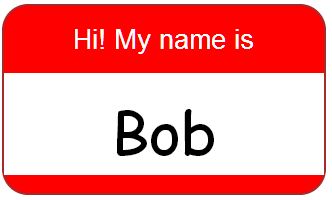
\includegraphics[height=5.0cm]{images/SS3.png}
\caption[
  Ausgangsbeispiel von der Trennung von Darstellung und Inhalt bei Shadow-DOM \citereset \autocite{Cooney.2013}
]{Ausgangsbeispiel von der Trennung von Darstellung und Inhalt bei Shadow-DOM}
\label{fig:3_ShadowDom2}
\end{figure}

Dadurch, dass dem DOM-Tree Kapselung fehlt, ist die gesamte Struktur des Namensschildes im Dokument sichtbar. Wenn beispielsweise externe Elemente auf der Webseite dieselben Klassennamen verwenden, würden diverse CSS-Klassen überschrieben werden.

\begin{enumerate}
\litem{Verstecken von Darstellungsdetails} \hfill \\
Semantisch gibt es nur zwei wichtige Informationen bei diesem Beispiel:
\begin{enumerate}
\item Es ist ein Namensschild
\item Der Name ist \glqq Bob\grqq .
\end{enumerate}
Daraus wird das Markup erstellt, das semantisch näher bei der gewünschten Information ist (siehe Code-Beispiel \ref{lst:3_ShadowDomBasic3}).

\begin{lstlisting}[language=HTML, caption={[Darstellung des Markups mit der gewünschten Information ohne Darstellung \citereset \autocite{Cooney.2013}] Darstellung des Markups mit der gewünschten Information ohne Darstellung}, label={lst:3_ShadowDomBasic3}, escapeinside={@}{@}]
<div id="nameTag">Bob</div>
\end{lstlisting}

Des Weiteren wird sämtlicher Code, der der Darstellung dient, in ein \lstinline|<template>|-Element gepackt (siehe Code-Beispiel \ref{lst:3_ShadowDomBasic4}). Dies ist notwendig um sämtliche Darstellungsdetails von dem eigentlichen Inhalt trennen zu können.

\begin{lstlisting}[language=HTML, caption={[Darstellung des Markups mit der gewünschten Information mit Hilfe von einem Template \citereset \autocite{Cooney.2013}] Darstellung des Markups mit der gewünschten Information mit Hilfe von einem Template}, label={lst:3_ShadowDomBasic4}, escapeinside={@}{@}]
<div id="nameTag">Bob</div>
<template id="nameTagTemplate">
  <style>
    .outer {
      border: 2px solid brown;
      border-radius: 1em;
      background: red;
      font-size: 20pt;
      width: 12em;
      height: 7em;
      text-align: center;
    }
    .boilerplate {
      color: white;
      font-family: sans-serif;
      padding: 0.5em;
    }
    .name {
      color: black;
      background: white;
      font-family: "Marker Felt", cursive;
      font-size: 45pt;
      padding-top: 0.2em;
    }
  </style>
  <div class="outer">
    <div class="boilerplate">
      Hi! My name is
    </div>
    <div class="name">
      Bob
    </div>
  </div>
</template>
\end{lstlisting}

Zu diesem Zeitpunkt wird \glqq Bob\grqq\ das einzige sein, das gerendert wird. Das Template enthält sämtlichen Code der Darstellung und muss nun beispielsweise mit JavaScript hinzugefügt werden. In Code-Beispiel \ref{lst:3_ShadowDomBasic5} auf Seite \pageref{lst:3_ShadowDomBasic5} wird zuerst eine Shadow-Root am Element \lstinline|<div id=nameTag></div>| erstellt. Danach wird nach dem Template gesucht und der Inhalt dieses Templates an die Shadow-Root angefügt.

\begin{lstlisting}[language=JavaScript, caption={[Hinzufügen des Inhalts eines Templates in eine Shadow-Root \citereset \autocite{Cooney.2013}] Hinzufügen des Inhalts eines Templates in eine Shadow-Root}, label={lst:3_ShadowDomBasic5}, escapeinside={@}{@}]
<script>
  var shadow = document.querySelector('#nameTag').createShadowRoot();
  var template = document.querySelector('#nameTagTemplate');
  shadow.appendChild(template.content);
</script>
\end{lstlisting}

Da nun eine Shadow-Root mit Markup vorhanden ist, wird das Namensschild wieder korrekt angezeigt. Wenn das Element mit Hilfe der Entwickler-Tools im Browser inspiziert wird, wird nur die gewünschte Information ohne Darstellungselemente angezeigt. Dies zeigt, dass durch die Verwendung von Shadow-DOM sämtliche Darstellungendetails im Shadow-DOM gekapselt wurden und von außen nicht erreichbar sind.

\litem{Trennung von Inhalt und Darstellung} \hfill \\
Mit Hilfe von Code-Beispiel \ref{lst:3_ShadowDomBasic4} und \ref{lst:3_ShadowDomBasic5} werden sämtliche Darstellungsdetails versteckt, jedoch wurde der Inhalt noch nicht mit der Darstellung getrennt. Wenn beispielsweise der Name des Namensschildes ausgetauscht werden müsste, müsste dies an zwei Stellen gemacht werden: Einerseits an der Stelle im Template und andererseits an der Stelle des \lstinline|<div id=nameTag></div>|-Elements.

Um den tatsächlichen Inhalt von sämtlichen Darstellungen zu trennen, muss eine Komposition von Elementen benutzt werden. Das Namensschild setzt sich einerseits aus dem roten Hintergrund mit den \glqq Hi! My name is\grqq -Text zusammen und andererseits aus dem Namen der Person.

Als Programmiererin beziehungsweise Programmierer einer Komponente kann entschieden werden, wie die Komposition des erstellten Elements funktionieren soll. Mit Hilfe des \lstinline|<content>|-Elements können Kompositionen erstellt werden. Dieses Element erstellt einen \glqq Insertion-Point\grqq\ in der Darstellung und sucht Inhalte aus dem Shadow-Host, die an dieser Stelle angezeigt werden sollten.

\begin{lstlisting}[language=HTML, caption={[Erweiterung des Code-Beispiels \ref{lst:3_ShadowDomBasic4} mit dem <content>-Element \citereset \autocite{Cooney.2013}] Erweiterung des Code-Beispiels \ref{lst:3_ShadowDomBasic4} mit dem <content>-Element}, label={lst:3_ShadowDomBasic6}, escapeinside={@}{@}]
<div id="nameTag">Bob</div>
<template id="nameTagTemplate">
  <style>
    .outer {
      border: 2px solid brown;
      border-radius: 1em;
      background: red;
      font-size: 20pt;
      width: 12em;
      height: 7em;
      text-align: center;
    }
    .boilerplate {
      color: white;
      font-family: sans-serif;
      padding: 0.5em;
    }
    .name {
      color: black;
      background: white;
      font-family: "Marker Felt", cursive;
      font-size: 45pt;
      padding-top: 0.2em;
    }
  </style>
  <div class="outer">
    <div class="boilerplate">
      Hi! My name is
    </div>
    <div class="name">
      <content></content>
    </div>
  </div>
</template>
\end{lstlisting}

In Code-Beispiel \ref{lst:3_ShadowDomBasic6} auf Seite \pageref{lst:3_ShadowDomBasic6} wird das Namensschild mit dem vom Shadow-Host projizierten Inhalt in das \lstinline|<content>|-Element gerendert. Dies vereinfacht die Struktur des Dokuments, da der Name nur noch an einer Stelle vorhanden ist. Müsste nun der Name aktualisiert werden, wäre das mit folgender Methode möglich: \lstinline|document.querySelector('#nameTag').textContent = 'Shellie';|.

Das Namensschild wird automatisch nach Zuweisung eines neuen Namens aktualisiert, da der Inhalt vom Namensschild in das \lstinline|<content>|-Element projiziert wird. Somit wurde die Trennung von Inhalt und Darstellung erreicht.
\end{enumerate}

\subsubsection{HTML Imports}
\label{sec:3_WC_Imports}

Es gibt eine Vielzahl von Möglichkeiten, wie man diverse Ressourcen lädt. Für JavaScript gibt es beispielsweise den \lstinline|<script src=''>|-Tag, für CSS gibt es den \lstinline|<link rel='stylesheet'>|-Tag. Weiters gibt es eigene Tags für Bilder, Video, Audio, etc. Die meisten Web-Inhalte haben einen einfachen, deklarativen Weg sie zu laden. HTML hingegen besitzt keinen standardisierten Weg. Zurzeit gibt es folgende Weg um HTML zu laden:
\begin{enumerate}
\item \lstinline|<iframe>|
\item AJAX
\item \lstinline|<script type='text/html'>|
\end{enumerate}

Jede dieser Methoden bringt seine Vor- und Nachteile mit sich und keine dieser Methoden ist eine standardisierte Weise, wie man externes HTML lädt.

HTML-Imports bieten einen standardisierten Weg, wie man ein HTML-Dokument in ein anderes HTML-Dokument lädt. Ein HTML-Import ist des Weiteren nicht auf Markup limitiert, sondern es kann auch CSS, JavaScript, etc. beinhalten. Listing \ref{lst:3_Imports_Basic1} auf Seite \pageref{lst:3_Imports_Basic1} zeigt, wie man ein lokales HTML-Dokument lädt.

\begin{lstlisting}[language=HTML, caption={Laden eines lokalen HTML-Dokuments}, label={lst:3_Imports_Basic1}, escapeinside={@}{@}]
<head>
  <link rel="import" href="path/to/imports/car.html"
</head>
\end{lstlisting}

Die URL eines Imports nennt man auch \glqq Import-Stelle\grqq . Um Inhalt von einer anderen Domain zu laden, muss die Import-Stelle CORS\footnote{Cross-Origin Resource Sharing} aktiviert sein. Listing \ref{lst:3_Imports_Basic2} auf Seite \pageref{lst:3_Imports_Basic2} zeigt, wie man ein externes HTML-Dokument lädt.

\begin{lstlisting}[language=HTML, caption={Laden eines externen HTML-Dokuments}, label={lst:3_Imports_Basic2}, escapeinside={@}{@}]
<head>
  <!-- Resources on other origins must be CORS-enabled. -->
  <link rel="import" href="http://example.com/car.html">
</head>
\end{lstlisting}

Der Netzwerk-Stack des Browsers entfernt sämtliche Duplikate bezüglich Requests von derselben URL. Dies bedeutet, dass bei Importe, die dieselbe URL haben, nur einmal aufgerufen werden.

\textbf{Ressourcen bündeln}

Importe stellen Konventionen bereit um HTML, CSS, JavaScript etc. bündeln zu können, damit sie als eine Datei lieferbar sind. Dies ist eine sehr wesentliche und mächtige Eigenschaft von HTML-Importe. Durch die Funktionen, die HTML-Importe bereitstellen, ist es möglich, eine Web-Applikation in einzelne, logische Segmente aufzuteilen und dem Endbenutzer dennoch nur eine URL geben zu müssen.

Ein sehr gutes Beispiel für einen sinnvollen Einsatz von HTML-Importe wäre Bootstrap\footnote{Mehr Information zu Dojo Toolkit unter \href{http://getbootstrap.com/}{http://getbootstrap.com/}}. Bootstrap besteht aus individuellen CSS- und JavaScript-Dateien, sowie Fonts. Darüber hinaus benötigt es für die bereitgestellten Plugins JQuery. Listing \ref{} auf Seite \pageref{} zeigt, wie man Bootstrap auf mehrere Dokumente aufteilen und laden könnte.

\begin{lstlisting}[language=HTML, caption={Inkludierung von Bootstrap mit Hilfe von einem HTML-Import}, label={lst:3_Imports_Basic3}, escapeinside={@}{@}]
<!-- main.html -->
<head>
  <link rel="import" href="bootstrap.html">
</head>

<!-- bootstrap.html -->
<link rel="stylesheet" href="bootstrap.css">
<link rel="stylesheet" href="fonts.css">
<script src="jquery.js"></script>
<script src="bootstrap.js"></script>
<script src="bootstrap-tooltip.js"></script>
<script src="bootstrap-dropdown.js"></script>
...
\end{lstlisting}

\textbf{Load/Error Event-Handling}
Das \lstinline|<link>|-Element feuert ein \glqq Load\grqq -Event, wenn ein HTML-Import erfolgreich geladen wurde und ein \glqq Error\grqq -Event, wenn dies nicht der Fall ist. Listing \ref{lst:3_Imports_Basic4} auf Seite \pageref{lst:3_Imports_Basic4} zeigt ein Beispiel von Error-Handling bei HTML-Importe.

\begin{lstlisting}[language=HTML, caption={Error-Handling bei HTML-Importe}, label={lst:3_Imports_Basic4}, escapeinside={@}{@}]
<head>
  <script>
  function handleLoad(e) {
    console.log('Loaded import: ' + e.target.href);
  }
  function handleError(e) {
    console.log('Error loading import: ' + e.target.href);
  }
</script>

  <link rel="import" href="car.html" onload="handleLoad(event)" onerror="handleError(event)">
</head>
\end{lstlisting}

Ein wichtiger Punkt bei dem in Listing \ref{lst:3_Imports_Basic4} gezeigten Beispiel ist, dass die Funktionen vor dem Import definiert wurden. Der Browser versucht einen HTML-Import dann zu laden, wenn er dem Tag begegnet. Wenn zu diesem Zeitpunkt die Funktionen noch nicht existieren, würden Fehler in der Konsole ausgegeben werden, da die Funktionsnamen noch \lstinline|undefined| sind.

\textbf{Benutzung des Inhalts eines Imports}
Wenn man einen HTML-Import benutzt, bedeutet dies nicht, dass an der Stelle, wo der Import-Befehl geschrieben  wird, der Inhalt des Imports platziert wird. Vielmehr bedeutet es, dass der Browser das zu importierende Dokument analysiert und es lädt, um es dann für weitere Verwendung bereit zu haben.\todo{umschreiben} Wenn man den Inhalt eines Imports erreichen will, da es beispielsweise gewisse \lstinline|<template>|-Elemente beinhaltet, muss man dafür JavaScript verwenden. Listing \ref auf Seite \pageref{} holt sich den Inhalt eines HTML-Imports. Die importierte Datei (warnings.html) beinhaltet diverses gestaltete Markup, was in der Hauptseite (main.html) verwendet werden sollte. Des Weiteren wird nur ein spezieller Teil des Imports verwendet, nämlich das \lstinline|<div>|-Element mit der Klasse \lstinline|warning|. Der restliche Inhalt des importierten HTML-Dokuments bleibt inaktiv und wird nicht vom Browser gerendered.

\begin{lstlisting}[language=JavaScript, caption={Klonen des Inhalts eines HTML-Imports}, label={lst:3_Imports_Basic5}, escapeinside={@}{@}]
<!-- warnings.html -->
<div class="warning">
  <style scoped>
    h3 {
      color: red;
    }
  </style>
  <h3>Warning!</h3>
  <p>This page is under construction</p>
</div>

<div class="outdated">
  <h3>Heads up!</h3>
  <p>This content may be out of date</p>
</div>


<!-- main.html -->
<head>
  <link rel="import" href="warnings.html">
</head>
<body>
    <script>
    var link = document.querySelector('link[rel="import"]');
    var content = link.import;

    // Grab specific DOM from warning.html's document.
    var el = content.querySelector('.warning');

    document.body.appendChild(el.cloneNode(true));
  </script>
</body>
\end{lstlisting}

\textbf{JavaScript in einem zu importierendem Dokument}
Importe befinden sich nicht im Hauptdokument. Sie können als Satelliten zum Hauptdokument gesehen werden. Im zu importierenden Dokument kann der DOM vom Hauptdokument und sein eigenes DOM erreicht werden. Listing \ref{lst:3_Imports_Basic6} auf Seite \pageref{lst:3_Imports_Basic6} zeigt, wie das zu importierende Dokument eines seiner Stylesheets selbst im Hauptdokument hinzufügt. Wichtig hierbei ist, dass das zu importierende Dokument einerseits eine Referenz zum eigenen Dokument und andererseits eine Referenz zum Hauptdokument beinhaltet.

\begin{lstlisting}[language=JavaScript, caption={JavaScript im HTML-Import, um Inhalt automatisch im Hauptdokument hinzuzufügen}, label={lst:3_Imports_Basic6}, escapeinside={@}{@}]
<link rel="stylesheet" href="http://www.example.com/styles.css">
<link rel="stylesheet" href="http://www.example.com/styles2.css">
<script>
  // importDoc references this import's document
  var importDoc = document.currentScript.ownerDocument;

  // mainDoc references the main document (the page that's importing us)
  var mainDoc = document;

  // Grab the first stylesheet from this import, clone it,
  // and append it to the importing document.
  var styles = importDoc.querySelector('link[rel="stylesheet"]');
  mainDoc.head.appendChild(styles.cloneNode(true));
</script>
\end{lstlisting}

Ein Skript in einem Import kann entweder Code direkt ausführen, oder Funktionen bereitstellen, die dem importierenden Dokument zur Verfügung stehen. Grundregeln für JavaScript in einem HTML-Import sind folgende:
\begin{itemize}
\item Skripte im Import werden im Kontext des importierenden Dokuments aufgerufen. Das bedeutet, dass \lstinline|window.document| im Import-Dokument eine Referenz zum Dokument ist, dass die Datei importiert. Dies hat zur Folge, dass sämtliche Funktionen, die im Import-Dokument definiert werden zum \lstinline|window|-Objekt hinzugefügt werden. Weiters ist es nicht erforderlich \lstinline|<script>|-Blöcke im Hauptdokument hinzuzufügen, da sie ausgeführt werden.
\item Importe blocken den Browser nicht beim Parsen des Hauptdokuments. Dennoch werden Skripte in den Importen der Reihe nach verarbeitet.
\end{itemize}

\textbf{HTML-Importe im Zusammenhang mit Templates}
Ein sehr großer Vorteil, wenn diese beiden Unterpunkte von Web-Components zusammen verwendet werden ist, dass Skripte innerhalb eines Templates nicht beim Laden des zu importierenden Dokuments ausgeführt werden, sondern erst dann, wenn das Template aktiv wird, sprich dem DOM des Hauptdokuments hinzugefügt wird.

\textbf{HTML-Importe im Zusammenhang mit benutzerdefinierten Elementen}
Wenn man diese beiden Technologien vereint, muss sich der Benutzer, der beispielsweise ein fremdes, benutzerdefiniertes Element mit Hilfe eines HTML-Imports lädt, nicht um die Registrierung des Elements kümmern, da es bereits im zu importierenden Dokument gemacht werden kann.

\textbf{Abhängigkeits-Management und Sub-Importe}
Sub-Importe sind vor allem dann vom Vorteil, wenn eine Komponente wiederverwendbar oder erweitert werden soll. Beispielsweise kann man JQuery als eine Komponente ansehen und sie als HTML-Import definieren. Wenn man mehrere, benutzerdefinierte Elemente mit Hilfe von JQuery entwickelt und sie anderen zur Verfügung stellt, werden die Abhängigkeiten für sämtliche Elemente automatisch geladen. Nimmt man an, das man drei benutzerdefinierte Elemente lädt, wobei jedes einzelne Element an sich JQuery als Abhängigkeit mittels HTML-Import geladen hat, wird JQuery trotzdem nur ein einziges Mal im Hauptdokument geladen.




HTML Importe
To detect support, check if .import exists on the <link> element:

function supportsImports() {
  return 'import' in document.createElement('link');
}

if (supportsImports()) {
  // Good to go!
} else {
  // Use other libraries/require systems to load files.
}
Browser support is still in the early days. Chrome 31 was the first browser to see an implementation. Since then, Chrome 36 was update with the latest spec. You can enable the flag by turning on Enable experimental Web Platform features in about:flags in Chrome Canary.



\subsection{Google Polymer}
\label{sec:3_Polymer}
\todo[inline]{Unterscheidung zwischen predefined Elements, self-written custom Elements und Benutzung von Elementen}
\todo[inline]{Nesting von Elements bzw. Reuse beispielhaft zeigen}




\iffalse
%STACKOVERFLOW POLYMER
In general, Polymer is a framework that aims to use (and show how to use) Web Components. It's foundation is Custom Elements (e.g. everything you build is a web component) and it evolves as the web evolves. To that end, we only support the latest version of the modern browsers.

I'll use this image to describe Polymer's entire architecture stack:
%polymers architecture http://i.stack.imgur.com/Ksn6s.png

RED layer: We get tomorrow's web through a set of polyfills. Keep in mind, those libraries go away over time as browsers adopt the new APIs.

YELLOW layer: Sprinkle in some sugar with polymer.js. This layer is our opinion on how to use the spec'd APIs, together. It also adds things like data-binding, syntatic sugar, change watchers, published properties...We think these things are helpful for building web component-based apps.

GREEN: The comprehensive set of UI components (green layer) is still in progress. These will be web components that use all of the red + yellow layers.

%STACKOVERFLOW END

How is Polymer different from Angular JS Directive? (Fundamentally and technologically)

Polymer (and more correctly, Shadow DOM) create the ability to not only compose bits of HTML, but to encapsulate them as well. This is a fundamentally new capability and one that can be used with any other templating system or framework to enhance their power.

In terms of templating/interpolation, Polymer uses MDV which does bi-directional data binding in a similar way to Angular for older browsers, but in newer runtimes can take advantage of Mutation Observers and eventually Object.observe() to help speed up change detection and propagation.
\fi



Ein Beispiel für ein vordefiniertes Element der Google-Polymer Bibliothek wäre das \lstinline|<polymer-ajax>|-Element. Es erscheint in erster Linie als nicht sehr nützlich, jedoch versucht es, einen Standard für Entwickler bereitzustellen, um Ajax-requests zu erstellen beziehungsweise abzuwickeln. Dieses Element ist ähnlich zu folgender Funktion: \lstinline|\$.ajax()|\footnote{Mehr Information zur jQuery.ajax-Funktion unter \href{http://api.jquery.com/jQuery.ajax/}{http://api.jquery.com/jQuery.ajax/}}. Der Unterschied zwischen den beiden Möglichkeiten, einen Ajax-Request abzuwickeln, ist, dass die \lstinline|\$.ajax()|-Methode Abhängigkeiten besitzt, wohingegen die \lstinline|<polymer-ajax>|-Methode vollkommen unabhängig ist.

\subsection{Konklusion}
\label{sec:3_Konklusion}



